%Set document format
\documentclass[11pt]{article}
\usepackage[margin=1in]{geometry}

%Set up packages
\usepackage{amsmath,amssymb,amsthm}
\usepackage{graphicx}
\usepackage{textcomp, gensymb}
\usepackage{float}
\usepackage{pdfpages}
\usepackage[hidelinks]{hyperref}
\usepackage{cancel}
\usepackage{subcaption}
\usepackage{caption}

\newcommand{\bm}{\boldsymbol}
\newcommand{\bI}{\mathbb{I}}
\newcommand{\bR}{\mathbb{R}}

\setlength\parindent{0pt}


\title{\bf OF-1 Report : \\[2mm] Computational Simulations of a Lid-driven Cavity}
\author{Terry Murray, Nicole Olvera, Andres Suniaga}
\date{02/11/2025}

\begin{document}
\maketitle

\noindent\makebox[\textwidth]{\rule{\textwidth}{0.2pt}}
\tableofcontents
\noindent\makebox[\textwidth]{\rule{\textwidth}{0.2pt}}
\pagebreak

\section{Introduction}
The incompressible, constant properties steady form of the Navier-Stokes equations is considered for the case of a 2D lid driven cavity with height = H, length = L, and lid velocity = U. 
The nondimensional forms of the continuity and momentum equations is recorded. After visualizing the solution for Re = 10, we experiment with the grid size to compare wallclock times with the refined solutions. 
We then estimate the relationship between wallclock time and the total number of grid points. We compute and plot the nondimensional stress along the lid at Reynolds numbers between 10 and 500. 
Finally, we compute the resulting force on the lid apect ratios 1/2, 1, and 2 and Reynolds numbers between 10 and 500. "TBR"
\section{Nondimensional Navier-Stokes equations}

\pagebreak

\section{Flow at Re = 10}

\subsection{Plots of Velocity}

\subsection{Solution Refinement}
\begin{figure}[H]
   \centering
   \begin{subfigure}{0.495\linewidth}
      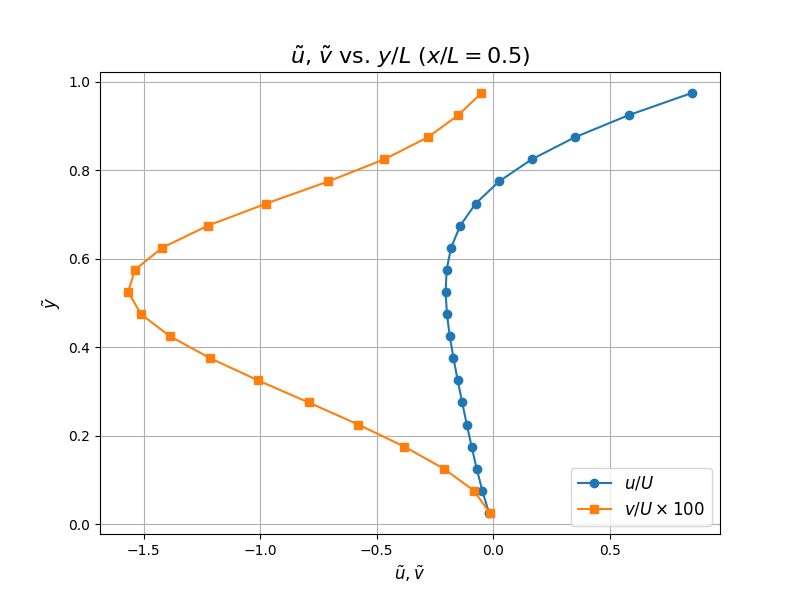
\includegraphics[width=\textwidth]{images/Velocity_Component_Plot_for_gridsize_20x20.png}
      \caption{Original}
   \end{subfigure}
   \begin{subfigure}{0.495\linewidth}
      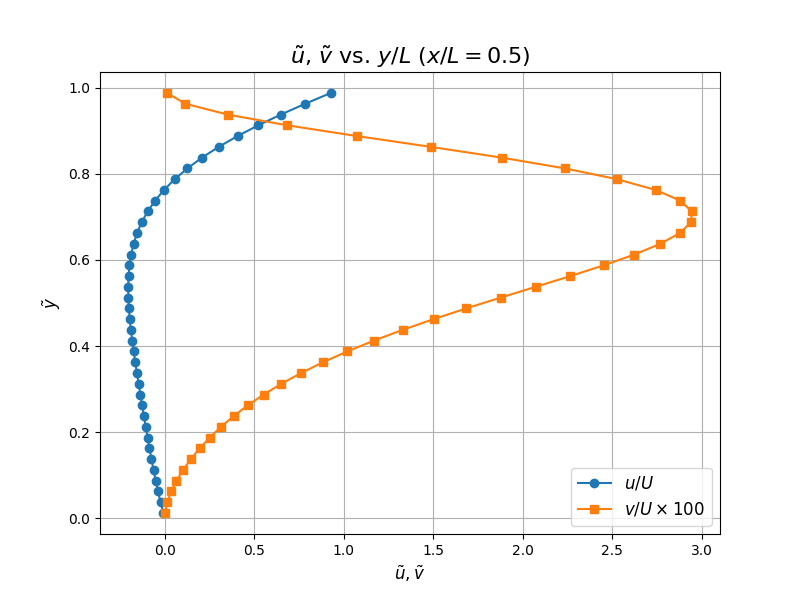
\includegraphics[width=\textwidth]{images/Velocity_Component_Plot_for_gridsize_40x40.png}
      \caption{First Refinement}
   \end{subfigure}
   \vspace{5mm}

   \begin{subfigure}{0.495\linewidth}
      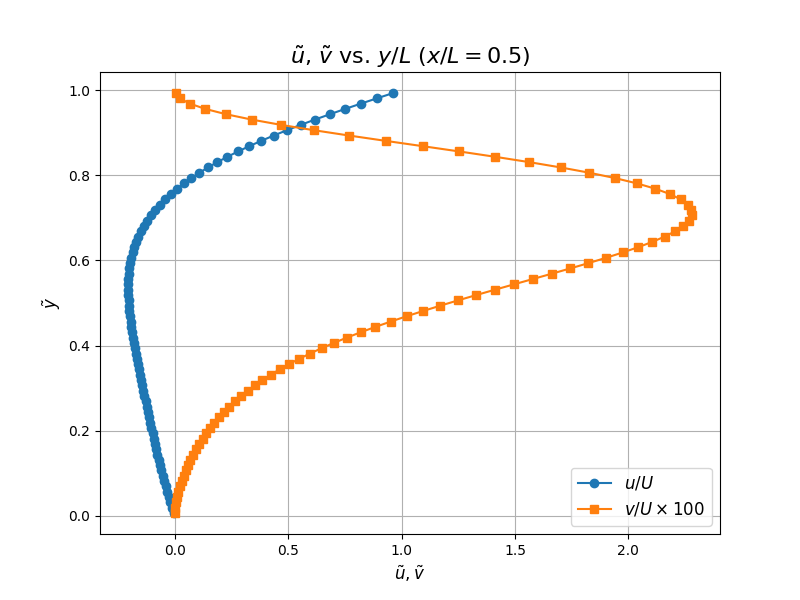
\includegraphics[width=\textwidth]{images/Velocity_Component_Plot_for_gridsize_80x80.png}
      \caption{Third Refinement}
   \end{subfigure}
   \begin{subfigure}{0.495\linewidth}
      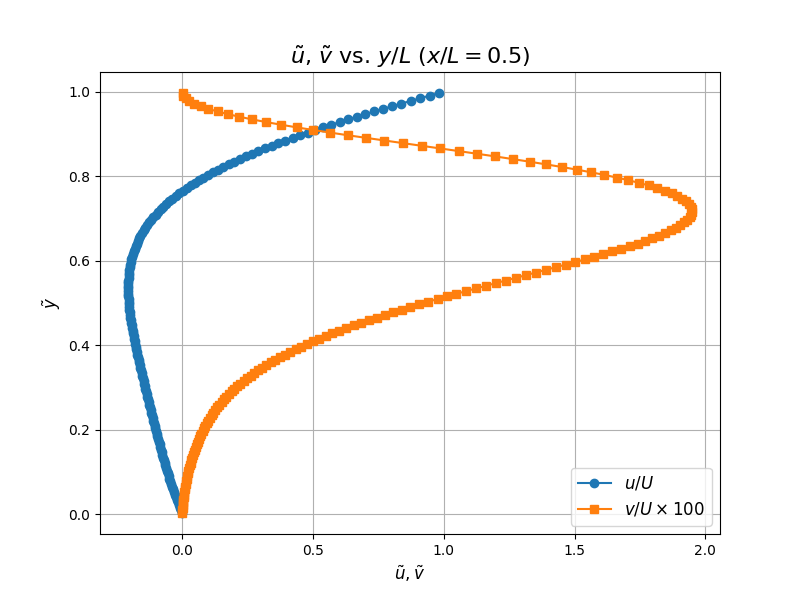
\includegraphics[width=\textwidth]{images/Velocity_Component_Plot_for_gridsize_160x160.png}
      \caption{Fourth Refinement}
   \end{subfigure}
   \vspace{2.5mm}

   \caption{Effect of increased gridsize and decreased time step size on $\tilde{u}$, $\tilde{v}$ vs. $\tilde{y}$}
   \label{velocityrefine}
\end{figure}

\begin{figure}[H]
   \centering
   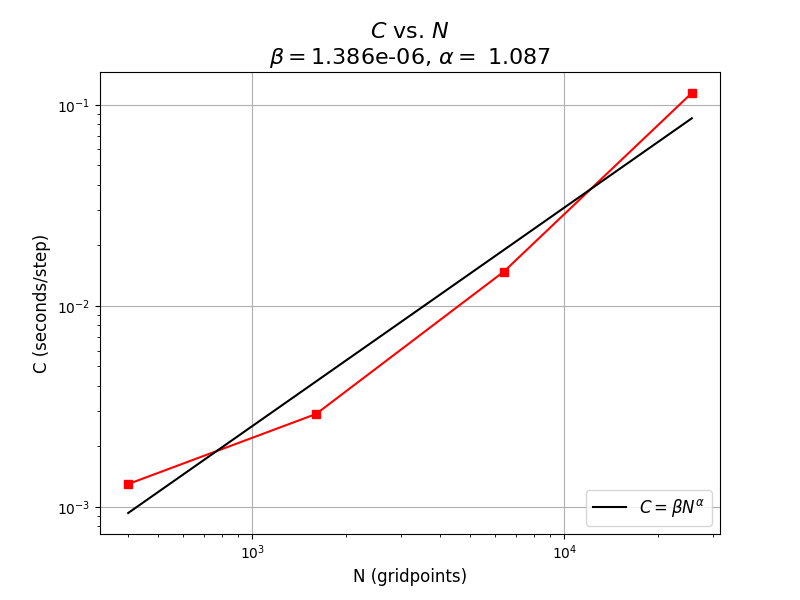
\includegraphics[width=0.85\textwidth]{images/Refinement_Measure.png}
   \caption{Execution time per step $C$ increases with higher gridpoints $N$}
   \label{timerefine}
\end{figure}

\begin{center}
   \fbox{\begin{minipage}{0.9\textwidth}
      \textbf{Q:} What can you conclude about the increase in wallclock time as you refine the grid?
   \end{minipage}}
\end{center}

\textbf{A:} Higher refinement will take longer per iteration than at lower refinement. It is clear in Fig. \ref{timerefine} with our estimate of $\alpha = 1.087$ in the fit $C = \beta N^{\alpha}$ that with an order of magnitude increase in gridpoints there is an order of magnitude increase in the execution time per step.

\pagebreak

\section{Force on the Lid}

\section{Conclusion}


\pagebreak
\appendix
\pagenumbering{gobble} 
\begin{center}
\vspace*{\fill}
   \Huge \bf Appendix 
\vspace*{\fill}
\end{center}
\pagebreak 

\hypertarget{code}{}
\section{Code}
PDF of code starts on next page.

\end{document}